\documentclass[UTF-8]{article}
\usepackage{amsmath}
\usepackage{amssymb}
\usepackage{float}
\usepackage{graphicx}
\usepackage{epstopdf}
\usepackage{inputenc}
\usepackage{geometry}
\usepackage{pgfplots} 
\usepackage{listings}
\usepackage{enumerate}
\usepackage{lipsum}  
\usepackage{color}
\usepackage[colorlinks=true, urlcolor=blue, linkcolor=blue]{hyperref}
\geometry{left=2.5cm,right=2.5cm,top=2.5cm,bottom=2.5cm}

\definecolor{codegreen}{rgb}{0,0.6,0}
\definecolor{codegray}{rgb}{0.5,0.5,0.5}
\definecolor{codepurple}{rgb}{0.58,0,0.82}
\definecolor{backcolour}{rgb}{0.9,0.9,0.92}

\lstdefinestyle{mystyle}{
    backgroundcolor=\color{backcolour},   
    commentstyle=\color{codegreen},
    keywordstyle=\color{blue},
    numberstyle=\tiny\color{codegray},
    stringstyle=\color{codepurple},
    basicstyle=\ttfamily\footnotesize,
    breakatwhitespace=false,         
    breaklines=true,                 
    captionpos=b,                    
    keepspaces=true,                 
    numbers=left,                    
    numbersep=5pt,                  
    showspaces=false,                
    showstringspaces=false,
    showtabs=false,                  
    tabsize=2
}

\lstset{style=mystyle}


\title{High Performance Computing Proseminar 2024 \\
    \large Assignment 1} %exchange for assignment number

\author{Sebastian Bergner}
\begin{document}
    
    \maketitle
    
    \section*{Exercise 1}
    This exercise consists in familiarizing yourself with SLURM job submission. 
    You received user credentials for the LCC3 cluster. If you did not change the default password, do so immediately. You are responsible for this
    account during this semester. 
    You can find information about LCC3 at \url{https://www.uibk.ac.at/zid/systeme/hpc-systeme/leo3/} and information about SLURM job submission at
    \url{https://www.uibk.ac.at/zid/systeme/hpc-systeme/common/tutorials/slurm-tutorial.html}. 
    Please run any benchmarks or heavy CPU loads only on the compute nodes, not on the login node. If you want to do some interactive
    experimentation, use an interactive job as outlined in the tutorial. Make sure to stop any interactive jobs once you are done. 
    
    \textbf{Tasks }
    \begin{itemize}
	    \item Study how to submit jobs in SLURM, how to check their state and how to cancel them.
	    \item Prepare a submission script that starts an arbitrary executable, e.g. /bin/hostname
	    \item In your opinion, what are the 5 most important parameters available when submitting a job and why? What are possible settings of these
	    parameters, and what effect do they have?
	    \item How do you run your program in parallel? What environment setup is required? 
	\end{itemize}	
	
	
	\begin{enumerate}
		\item Submiting jobs in SLURM consits of first writing a job file where the configuration is written in SLURM specific format. Afterwards we can submit the job using \verb|sbatch filename.sh|. To check their state we can either use \verb|squ| or \verb|squeue| where the latter shows all jobs from all users. \verb|scancel job-id| terminates the job with the according job-id.
		\item The following script measures the time required to execute \verb|/bin/hostname|.
		\begin{lstlisting}
#!/bin/bash

# Execute job in the partition "lva" unless you have special requirements.
#SBATCH --partition=lva
# Name your job to be able to identify it later
#SBATCH --job-name ps1
# Redirect output stream to this file (if the output is assumed to be larger put it in scratch)
#SBATCH --output=output.log
# Maximum number of tasks (=processes) to start in total
#SBATCH --ntasks=1
# Maximum number of tasks (=processes) to start per node
#SBATCH --ntasks-per-node=1
# Enforce exclusive node allocation, do not share with other jobs
#SBATCH --exclusive
/usr/bin/time -v /bin/hostname\end{lstlisting}

	\item The 5 most important parameters are (IMO)
	\begin{enumerate}[I]
		\item \verb|#SBATCH --time=...| which sets the time limit to the given argument (in this format: [[D-]HH:]MM[:SS]). For our purposes it is less important, but generally speaking it makes much sense to limit the duration. An example would be \verb|#SBATCH --time=1:30:00| which configures the job to run for 1.5 hours. If a job takes longer it'll be terminated.
		\item \verb|#SBATCH --exclusive| is mandatory if we want to make any meaningful (performance) measurement as it reserves the entire machine for this job. If other jobs would run here they could interfere with the cache or main memory access latencies.
		\item \verb|#SBATCH --output=outputfile.txt| (as well as error) pipes the output stream (or error stream) into an according file. This is useful for debugging textual outputs of our program we submitted.
		\item \verb|#SBATCH --mail-user=Karl.Mustermann@xxx.com| in combination with \verb|#SBATCH --mail-type=END,FAIL| is not mandatory but quite nice if we have a long running job and want to be notified whenever the job either terminates or fails. \verb|mail-type| supports the following types: BEGIN, END, FAIL, REQUEUE, STAGE\_OUT, TIME\_LIMIT, TIME\_LIMIT\_90, TIME\_LIMIT\_80, TIME\_LIMIT\_50, ARRAY\_TASKS. (Stage out \url{https://slurm.schedmd.com/burst_buffer.html})
		\item \verb|#SBATCH --job-name=name| may seem silly to put into this list but it is quite helpful to distinguish from other jobs especially if many are being executed simultaneously.
	\end{enumerate}

To run programs on several nodes in parallel utilizing the openMPI functionality we have to setup our configuration in the job file. The following parameters can be adjusted according to the system and the requirements:
\begin{lstlisting}[language=bash]
#!/bin/bash

#SBATCH --partition=lva
#SBATCH --job-name myjob
#SBATCH --output=output.log

#SBATCH --ntasks=10
#SBATCH --nodes=10

#SBATCH --exclusive

# load required modules
module load openmpi/3.1.6-gcc-12.2.0-d2gmn55 
mpiexec -n $SLURM_NTASKS ./somexec
\end{lstlisting}

\verb|ntasks| specifies the overall number of task that should be distributed. \verb|nodes| corresponds to the number of individual nodes (not NUMA's but rather machines) while \verb|ntasks-per-socket| specifies how many should run per NUMA node. \verb|ntasks-per-node| sets the tasks per node to a fixed number. And lastly \verb|cpus-per-task| can set the number of CPU's per each task (can occur that CPU's on separate nodes work on one task $\rightarrow$ unideal for latency and throughput). Afterwards I found out that it really only makes sense to set the ntasks and the nodes and orchestrate the location of each task using mpiexec's parameters bind-to and map-by.


	\end{enumerate}
	
    \section*{Exercise 2}
    This exercise consists in running an MPI microbenchmark in order to examine the impact of HPC topologies on performance.
    
    The OSU Micro-Benchmarks suite holds multiple benchmarks that measure low-level performance properties such as latency and bandwidth between MPI ranks (=processes). Specifically, for this exercise, we are interested in the point-to-point ones, which exchange messages between 2 MPI ranks.
    
    \textbf{Tasks}
    \begin{itemize}
    	\item Download and build the OSU Micro-Benchmarks available at \url{http://mvapich.cse.ohio-state.edu/download/mvapich/osu-micro-benchmarks-5.8.tgz}. Do not forget to set the compiler parameters for configure, e.g. ./configure CC=mpicc CXX=mpic++ ...
    	\item After building, submit SLURM jobs that run the osu\_latency and osu\_bw executables.
    	\item Create a table and figures that illustrate the measured data and study them. What effects can you observe?
    	\item Find out more about the hardware that you're running on, e.g. by using lstopo --of txt (available via module load hwloc). Modify your experiment such that the 2 MPI ranks are placed on
    	different cores of the same socket,
    	different sockets of the same node, and
    	different nodes.
    	\item Amend your table and figures to include these additional measurements. What effects can you observe? How can you verify rank placement without looking at performance?
    	\item How stable are the measurements when running the experiments multiple times?
    	\item Insert the measured time for latency (size 0) and bandwidth (size 1048576) into the comparison spreadsheet: \url{https://docs.google.com/spreadsheets/d/1p6d9F12EtykmI2-7MnHkg0U15UAtaCvWz8Ip92ZEsWo}
    \end{itemize}
    
    From the documentation of OSU (\url{https://mvapich.cse.ohio-state.edu/benchmarks/}):
    \begin{lstlisting}
osu_latency - Latency Test
The latency tests are carried out in a ping-pong fashion. The sender sends a message with a certain data size to the receiver and waits for a reply from the receiver. The receiver receives the message from the sender and sends back a reply with the same data size. Many iterations of this ping-pong test are carried out and average one-way latency numbers are obtained. Blocking version of MPI functions (MPI_Send and MPI_Recv) are used in the tests. 

osu_bw - Bandwidth Test
The bandwidth tests are carried out by having the sender sending out a fixed number (equal to the window size) of back-to-back messages to the receiver and then waiting for a reply from the receiver. The receiver sends the reply only after receiving all these messages. This process is repeated for several iterations and the bandwidth is calculated based on the elapsed time (from the time sender sends the first message until the time it receives the reply back from the receiver) and the number of bytes sent by the sender. The objective of this bandwidth test is to determine the maximum sustained date rate that can be achieved at the network level. Thus, non-blocking version of MPI functions (MPI_Isend and MPI_Irecv) are used in the test. 
\end{lstlisting}
    
    
    
    
    For building we first have to load all required modules (gcc and openmpi) then we can use configure with the flags CC=mpicc CXX=mpic++ and a proper --prefix=path where we have access to. Then we can build and install with \verb|make && make install|. After that the compiled binaries should be located in our specified path.
    
\begin{lstlisting}[language=bash]
#!/bin/bash

#SBATCH --partition=lva
#SBATCH --job-name ps1.1
#SBATCH --output=output1.log

#SBATCH --ntasks=2
#SBATCH --nodes=1

#SBATCH --exclusive

# load all required modules
module purge
module load openmpi/3.1.6-gcc-12.2.0-d2gmn55 

# executing
for i in {1..5}; do
echo $i
mpiexec --display-map --bind-to core --map-by core /home/cb76/cb761014/exercise1/osu-micro-benchmarks-5.8/executables/libexec/osu-micro-benchmarks/mpi/pt2pt/osu_latency
done
for i in {1..5}; do
echo $i
mpiexec --display-map --bind-to core --map-by core /home/cb76/cb761014/exercise1/osu-micro-benchmarks-5.8/executables/libexec/osu-micro-benchmarks/mpi/pt2pt/osu_bw
done
\end{lstlisting}

    \begin{figure}[H]
    	\centering
    	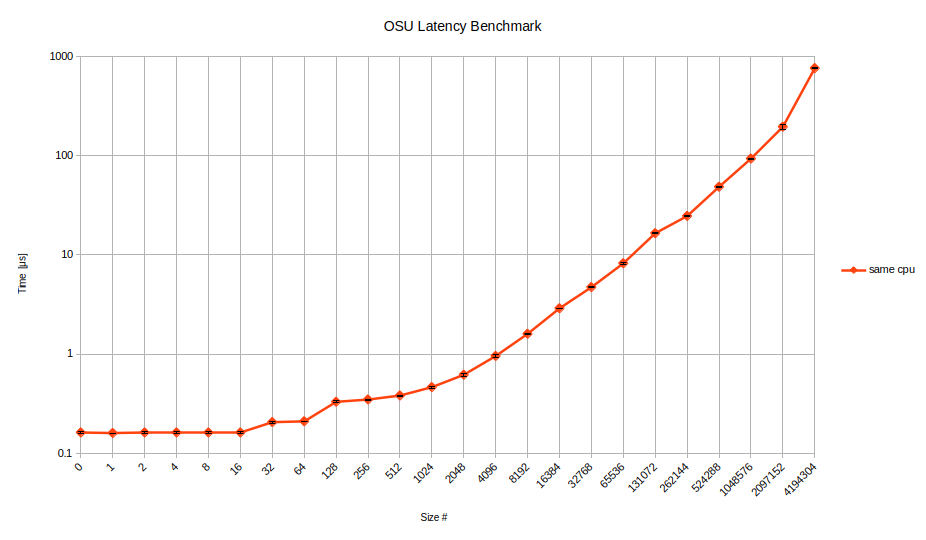
\includegraphics[width=0.9\linewidth]{01/plot_osu_latency_only_cpu.png}
    	\caption{OSU latency plot only cpu.}
    	\label{fig:plotosulatencycpu}
    \end{figure}
    
    In the above Fig. \ref{fig:plotosubwcpu} we can observe the latency remains constant until about a size of 16-32 (kB) which would correspond to the L1d cache, after that a slow incline can be seen until about 256-512 (kB) which again would fit the L2 cache after that we can see a steep increase in latency which could be the jump to L3 and later on after about 12MB, to main memory.
    
    \begin{figure}[H]
    	\centering
    	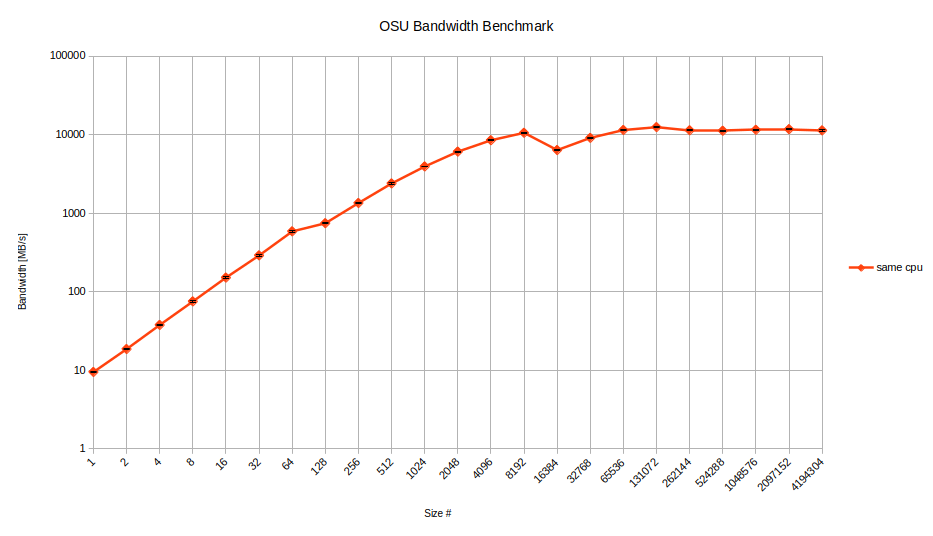
\includegraphics[width=0.9\linewidth]{01/plot_osu_bw_only_cpu.png}
    	\caption{OSU bandwidth plot only cpu.}
    	\label{fig:plotosubwcpu}
    \end{figure}
    
    Here in Fig. \ref{fig:plotosubwcpu} we can observe something similar we have a nice linear relationship until 64 (kB?) after that it slowly tapers off. Interestingly at a size of 8192 (kB) it reached its peak and remains at a rate of about 10GB/s.
    
    
    
    \begin{center}
    \begin{tabular}{|c|c|c|}
    	\hline
    	Size & Avg latency $\mu$s & Avg bandwidth MB/s \\
    	\hline
    	0 & 0.162 &  \\
    	\hline
    	1 & 0.16 & 9.514 \\
    	\hline
    	2 & 0.162 & 18.632 \\
    	\hline
    	4 & 0.162 & 37.798 \\
    	\hline
    	8 & 0.162 & 75.33 \\
    	\hline
    	16 & 0.162 & 151.436 \\
    	\hline
    	32 & 0.206 & 290.404 \\
    	\hline
    	64 & 0.21 & 587.482 \\
    	\hline
    	128 & 0.33 & 746.458 \\
    	\hline
    	256 & 0.348 & 1349.638 \\
    	\hline
    	512 & 0.382 & 2396.042 \\
    	\hline
    	1024 & 0.464 & 3939.186 \\
    	\hline
    	2048 & 0.618 & 6083.762 \\
    	\hline
    	4096 & 0.956 & 8495.482 \\
    	\hline
    	8192 & 1.598 & 10568.65 \\
    	\hline
    	16384 & 2.888 & 6370.756 \\
    	\hline
    	32768 & 4.714 & 9105.146 \\
    	\hline
    	65536 & 8.21 & 11464.932 \\
    	\hline
    	131072 & 16.492 & 12488.038 \\
    	\hline
    	262144 & 24.61 & 11369.246 \\
    	\hline
    	524288 & 48.462 & 11217.328 \\
    	\hline
    	1048576 & 93.19 & 11540.738 \\
    	\hline
    	2097152 & 195.026 & 11746.71 \\
    	\hline
    	4194304 & 759.64 & 11330.14 \\
    	\hline
    \end{tabular}
\end{center}
    





\begin{figure}[H]
	\centering
	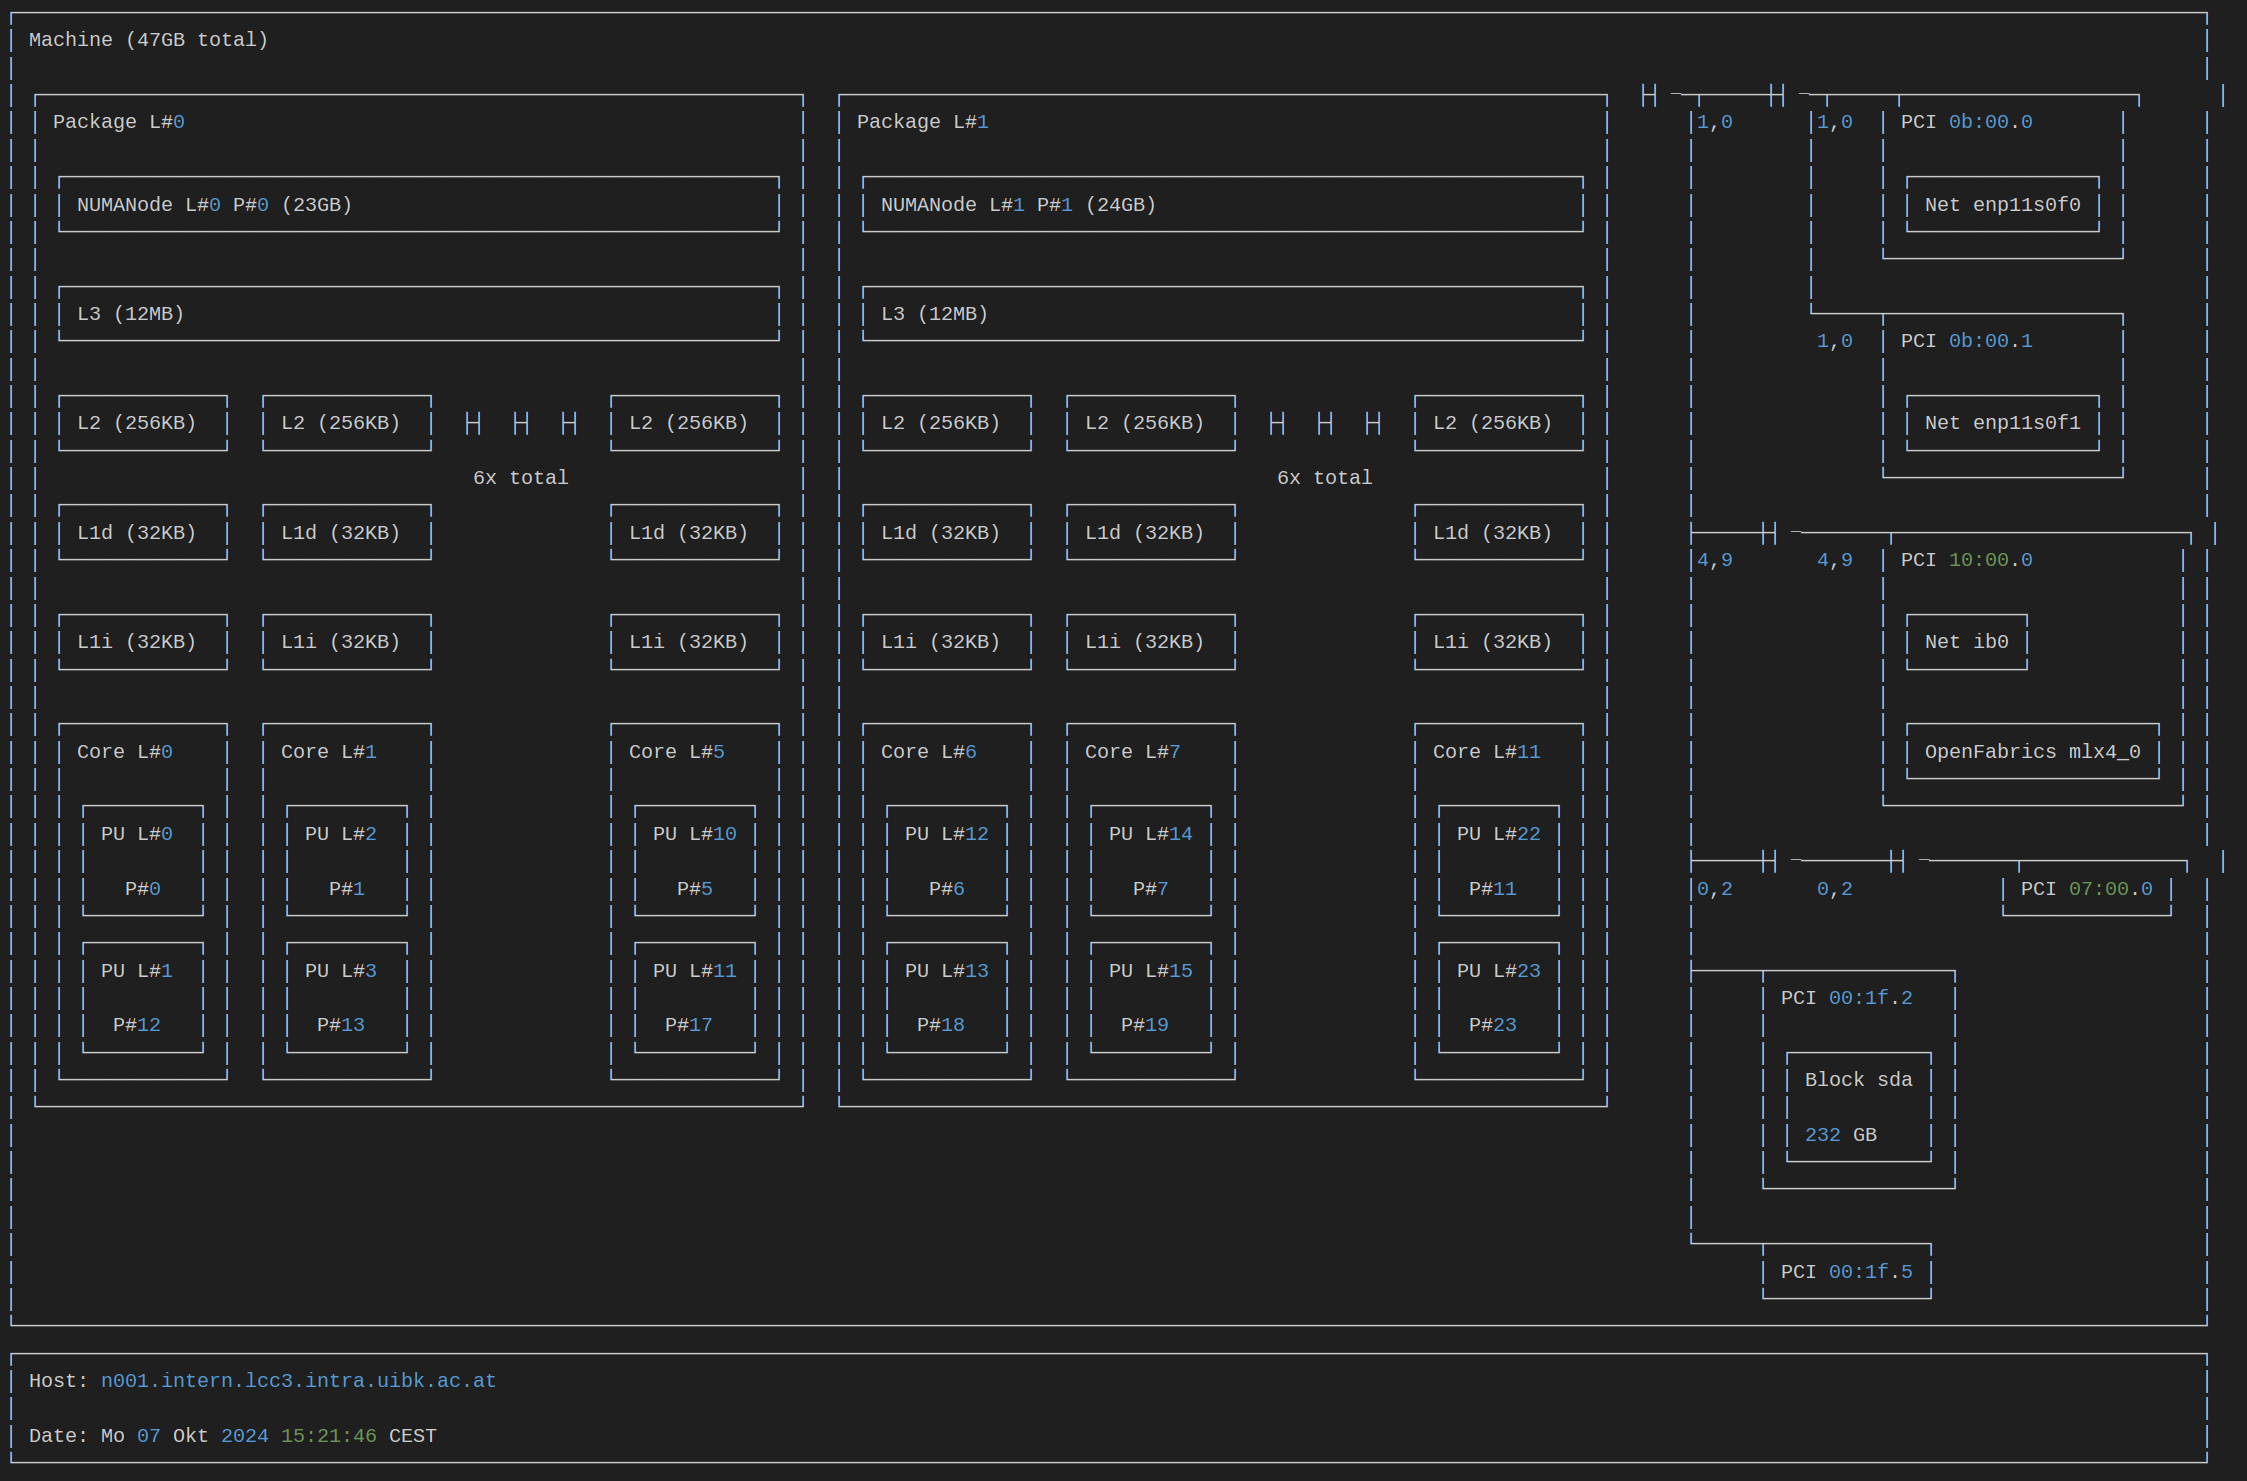
\includegraphics[width=0.7\linewidth]{01/lstopo}
	\caption{lstopo output.}
	\label{fig:lstopo}
\end{figure}

From the lstopo output we can infer that a node consists of 2 NUMA nodes (i.e. has 2 CPU sockets) with 23GB and 24GB of main memory. They both have the same cache architecture with 12MB of L3 cache. 256KB L2 per core cache and 32KB L1d and L1i caches. And we can see that a core consists of two processing units (hw core and hyperthreading/SMT). The nodes are interconnected using OpenFabrics interconnect (InfiniBand) and have two ethernet interfaces. (The login node has compared to the other nodes 32GB of memory per socket.)




\begin{figure}[H]
	\centering
	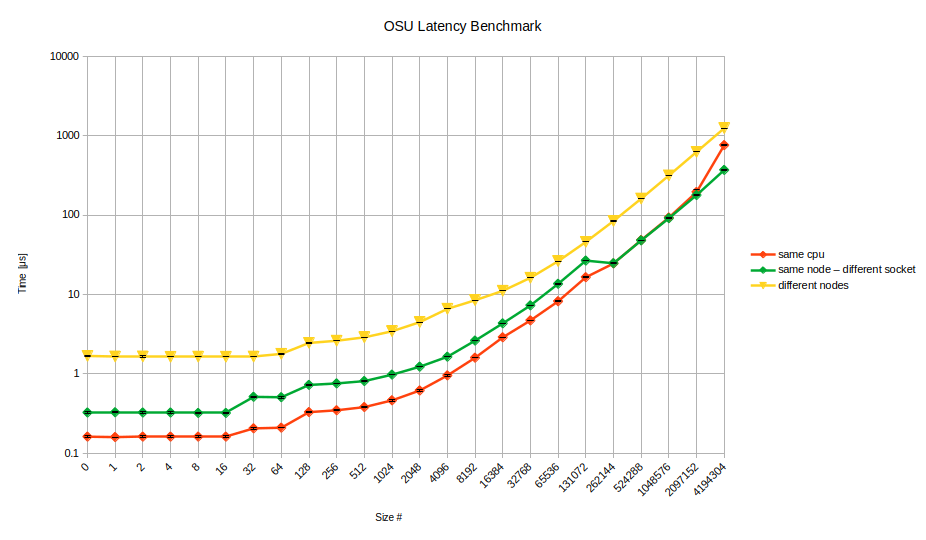
\includegraphics[width=0.9\linewidth]{01/plot_osu_latency}
	\caption{Plot of OSU latency benchmark output.}
	\label{fig:plotosulatency}
\end{figure}

From the latency benchmark Fig. \ref{fig:plotosulatency} a large difference between the CPU vs. rest can be seen. The relative difference is at first larger (up to $\times 10$) and gets smaller. Something unexpected is that the latency of the CPU bench gets larger than the different socket benchmark. Would be interesting to get to know the reason behind this.
    
\begin{figure}[H]
	\centering
	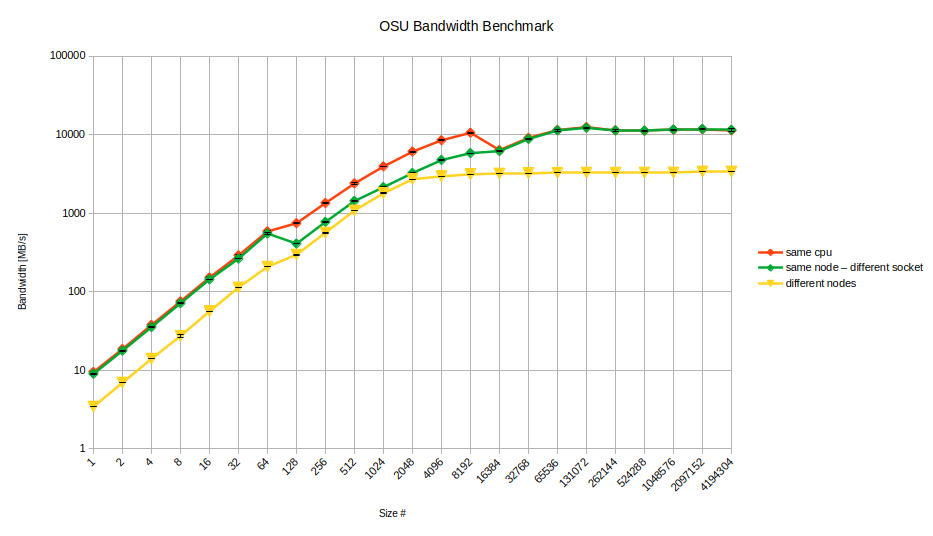
\includegraphics[width=0.7\linewidth]{01/plot_osu_bw}
	\caption{Plot of OSU bandwidth benchmark output.}
	\label{fig:plotosubw}
\end{figure}

For the bandwidth benchmark (Fig. \ref{fig:plotosubw}) we can observe that the throughput of the CPU and socket benchmark are quite similar. Both taper off to about 11 GB/s while the benchmark distributed on 2 separate nodes tapers off at about 3.4 GB/s which is considerably less.
So we could conclude that distance in distributed systems is a very relevant metric and if possible message passing should be kept to a minimum size and maximum time distance if possible. And to try and keep the tasks/jobs as close as possible to another (especially if they have to communicate a lot). Otherwise we decrease computational efficiency and extend the runtime of the program by multiple times.
\\

To verify rank placement we can utilize \verb|mpiexec --display-map| (\href{https://www.open-mpi.org/doc/v3.0/man1/mpiexec.1.php#:~:text=%2Ddisplay%2Dmap%2C%20%2D%2Ddisplay%2Dmap}{display-map - mpiexec man page}) in our job script. This displays the location of the tasks on the hardware.
\begin{lstlisting}
# different CPU cores
 Data for node: n001	Num slots: 2	Max slots: 0	Num procs: 2
Process OMPI jobid: [4154,1] App: 0 Process rank: 0 Bound: socket 0[core 0[hwt 0-1]]:[BB/../../../../..][../../../../../..]
Process OMPI jobid: [4154,1] App: 0 Process rank: 1 Bound: socket 0[core 1[hwt 0-1]]:[../BB/../../../..][../../../../../..]

# different Sockets
Data for node: n001	Num slots: 2	Max slots: 0	Num procs: 2
Process OMPI jobid: [8583,1] App: 0 Process rank: 0 Bound: socket 0[core 0[hwt 0-1]]:[BB/../../../../..][../../../../../..]
Process OMPI jobid: [8583,1] App: 0 Process rank: 1 Bound: socket 1[core 6[hwt 0-1]]:[../../../../../..][BB/../../../../..]



# Different Nodes (interestingly mpiexec is unable to display the "Bound" on the second node)
 Data for node: n002	Num slots: 1	Max slots: 0	Num procs: 1
Process OMPI jobid: [28289,1] App: 0 Process rank: 0 Bound: socket 0[core 0[hwt 0-1]]:[BB/../../../../..][../../../../../..]

Data for node: n003	Num slots: 1	Max slots: 0	Num procs: 1
Process OMPI jobid: [28289,1] App: 0 Process rank: 1 Bound: N/A
\end{lstlisting}


\begin{table}
	Measurements all in $\mu s$.
	\centering
	\begin{tabular}{|c|c|c|c|c|c|c|} 
		\hline
		Size    & $\mu$ Lat. CPU & $\sigma$ Lat. CPU & $\mu$ Lat. Socket & $\sigma$ Lat. Socket~ & $\mu$ Lat. Nodes & $\sigma$ Lat. Nodes  \\ 
		\hline
		0       & 0.162        & 0.004         & 0.326           & 0.005             & 1.684          & 0.005            \\ 
		\hline
		1       & 0.16         & 0             & 0.328           & 0.004             & 1.654          & 0.008            \\ 
		\hline
		2       & 0.162        & 0.004         & 0.326           & 0.005             & 1.656          & 0.026            \\ 
		\hline
		4       & 0.162        & 0.004         & 0.326           & 0.005             & 1.638          & 0.004            \\ 
		\hline
		8       & 0.162        & 0.004         & 0.322           & 0.004             & 1.648          & 0.004            \\ 
		\hline
		16      & 0.162        & 0.004         & 0.322           & 0.004             & 1.642          & 0.004            \\ 
		\hline
		32      & 0.206        & 0.005         & 0.514           & 0.005             & 1.65           & 0.007            \\ 
		\hline
		64      & 0.21         & 0             & 0.508           & 0.010             & 1.786          & 0.005            \\ 
		\hline
		128     & 0.33         & 0.007         & 0.726           & 0.008             & 2.454          & 0.008            \\ 
		\hline
		256     & 0.348        & 0.004         & 0.758           & 0.004             & 2.614          & 0.011            \\ 
		\hline
		512     & 0.382        & 0.004         & 0.812           & 0.004             & 2.888          & 0.008            \\ 
		\hline
		1024    & 0.464        & 0.011         & 0.978           & 0.008             & 3.444          & 0.005            \\ 
		\hline
		2048    & 0.618        & 0.017         & 1.232           & 0.004             & 4.484          & 0.008            \\ 
		\hline
		4096    & 0.956        & 0.034         & 1.644           & 0.005             & 6.6            & 0.014            \\ 
		\hline
		8192    & 1.598        & 0.008         & 2.624           & 0.005             & 8.466          & 0.011            \\ 
		\hline
		16384   & 2.888        & 0.021         & 4.33            & 0.014             & 11.12          & 0.007            \\ 
		\hline
		32768   & 4.714        & 0.034         & 7.286           & 0.015             & 16.236         & 0.011            \\ 
		\hline
		65536   & 8.21         & 0.165         & 13.626          & 0.068             & 26.314         & 0.037            \\ 
		\hline
		131072  & 16.492       & 0.260         & 26.744          & 0.140             & 45.936         & 0.027            \\ 
		\hline
		262144  & 24.61        & 0.273         & 24.748          & 0.333             & 84.4           & 0.411            \\ 
		\hline
		524288  & 48.462       & 0.771         & 47.968          & 0.385             & 161.268        & 0.029            \\ 
		\hline
		1048576 & 93.19        & 0.932         & 91.462          & 0.687             & 315.738        & 0.019            \\ 
		\hline
		2097152 & 195.026      & 12.984        & 178.528         & 1.06              & 624.568        & 0.070            \\ 
		\hline
		4194304 & 759.64       & 5.819         & 370.196         & 3.98              & 1243.174       & 0.287            \\
		\hline
	\end{tabular}
\end{table}


\begin{table}
	\centering
	Measurements all in $MB/s$.
	\begin{tabular}{|c|c|c|c|c|c|c|} 
		\hline
		Size    & $\mu$ Bw. CPU & $\sigma$ Bw. CPU & $\mu$ Bw. Socket & $\sigma$ Bw. Socket & $\mu$ Bw. Nodes & $\sigma$ Bw. Nodes  \\ 
		\hline
		0       &             &              &                &                 &               &                 \\ 
		\hline
		1       & 9.514       & 0.110        & 9.022          & 0.118           & 3.444         & 0.008           \\ 
		\hline
		2       & 18.632      & 0.354        & 17.77          & 0.256           & 6.974         & 0.023           \\ 
		\hline
		4       & 37.798      & 0.663        & 35.458         & 0.454           & 14.03         & 0.045           \\ 
		\hline
		8       & 75.33       & 1.248        & 71.428         & 1.078           & 27.404        & 1.051           \\ 
		\hline
		16      & 151.436     & 3.124        & 143.618        & 0.631           & 56.314        & 0.544           \\ 
		\hline
		32      & 290.404     & 7.547        & 264.164        & 2.439           & 113.484       & 0.251           \\ 
		\hline
		64      & 587.482     & 14.886       & 551.892        & 10.357          & 208.796       & 0.528           \\ 
		\hline
		128     & 746.458     & 5.328        & 410.014        & 3.271           & 297.122       & 4.872           \\ 
		\hline
		256     & 1349.638    & 25.323       & 774.53         & 5.609           & 566.312       & 8.173           \\ 
		\hline
		512     & 2396.042    & 43.719       & 1431.542       & 16.969          & 1083.606      & 10.124          \\ 
		\hline
		1024    & 3939.186    & 36.755       & 2145.924       & 23.387          & 1799.9        & 15.884          \\ 
		\hline
		2048    & 6083.762    & 63.182       & 3246.95        & 17.027          & 2712.14       & 6.580           \\ 
		\hline
		4096    & 8495.482    & 110.107      & 4760.958       & 27.490          & 2946.168      & 4.597           \\ 
		\hline
		8192    & 10568.65    & 62.968       & 5825.58        & 16.604          & 3128.782      & 5.183           \\ 
		\hline
		16384   & 6370.756    & 113.711      & 6188.69        & 90.301          & 3203.914      & 4.412           \\ 
		\hline
		32768   & 9105.146    & 119.976      & 8823.432       & 225.554         & 3245.912      & 1.133           \\ 
		\hline
		65536   & 11464.932   & 227.476      & 11327.316      & 190.221         & 3270.642      & 0.987           \\ 
		\hline
		131072  & 12488.038   & 262.564      & 12231.7        & 303.271         & 3282.504      & 0.866           \\ 
		\hline
		262144  & 11369.246   & 166.984      & 11306.872      & 177.802         & 3286.506      & 4.150           \\ 
		\hline
		524288  & 11217.328   & 124.078      & 11243.862      & 130.569         & 3294.292      & 0.497           \\ 
		\hline
		1048576 & 11540.738   & 123.555      & 11611.17       & 149.700         & 3296.104      & 0.779           \\ 
		\hline
		2097152 & 11746.71    & 106.510      & 11809.352      & 214.741         & 3395.628      & 0.069           \\ 
		\hline
		4194304 & 11330.14    & 260.713      & 11494.262      & 418.389         & 3396.388      & 0.014           \\
		\hline
	\end{tabular}
\end{table}

The measurements were all conducted 5 times and looking at the table/plots we can say the measurements are stable within $1-2 \%$ with one exception where the standard deviation is 6\% of the average which is not that much to invalidate the measurement.




\end{document}